% !TeX spellcheck = en_US
% !TeX encoding = UTF-8 

\documentclass[14pt,a4paper]{extarticle}

\usepackage[english]{babel}
\usepackage[utf8]{inputenc}
\usepackage{setspace} 
\usepackage[a4paper,
	left=30mm,
	right=10mm,
	top=20mm,
	bottom=20mm]{geometry}
\usepackage{amsmath}
\usepackage{amssymb}
\usepackage{amsthm}
\usepackage{graphicx} 
\usepackage{cite}
\usepackage{subfigure}
\usepackage{subcaption}
\usepackage{kprjHSE} 
\usepackage{listings}
\usepackage{tabu}
\usepackage{courier}

\lstset{
	frame=single,
	basicstyle=\ttfamily,
	breaklines=true,
	tabsize=4
}

\LabWork
\LabWorkNo{1}

\FirstAuthor{M.D.~Kirdin}
\FirstConsultant{A.~Tomat}
\SecondConsultant{M.~Zueva}
\discipline{Ordered Sets for Data Analysis}
\faculty{Faculty of Computer Science}
\chair{School of Data Analysis and Artificial Intelligence}
\chief{S.O.~Kuznetsov}
\workyear{2024}

\onehalfspacing

\begin{document}
	\maketitle
	
	\subsection*{Question 1}
	Consider a binary relation $R\subseteq A\times A$, where $A=\{a,\,b,\,c,\,d,\,e\}$, defined by following matrix:
	\begin{center}
	\begin{tabu}{ |X[c]|X[c]|X[c]|X[c]|X[c]|X[c]|}
		\hline
		 & a & b & c & d & e\\
		\hline
		a & 1 &  & 1 & 1 & 1\\
		\hline
		b & 1 & 1 &  &  & \\
		\hline
		c &  & 1 & 1 &  & 1\\
		\hline
		d &  &  & 1 & 1 & \\
		\hline
		e & 1 & 1 & 1 & 1 & 1\\
		\hline
	\end{tabu}
	\end{center}
	
	 \noindent\textbf{Task.} Determine whether $R$ has certain properties and explain why.
	 
	 \noindent\textbf{Solution.}
	 
	 \begin{enumerate}
	 	\item \textit{Reflexivity.} R is reflexive, since $R:\forall x\in A \,\,\, xRx$.
	 	\item \textit{Antireflexity.} R is not antireflexive, since $\exists x\in A: \lnot xR^{c}x$. For example, $x=a$. 
	 	\item \textit{Symmetricity.} R is not symmetric, since $\exists x,\, y\in A: xRy \implies \lnot yRx$. For example, $x=a,\, y=b$. 
	 	\item \textit{Asymmetricity.} R is not asymmetric, since $\exists x,\, y\in A: xRy \implies \lnot yR^{c}x$. For example, $x = a = y$.
	 	\item \textit{Antisymmetricity.} R is not antisymmetric, since $aRb\, \&\, bRa \implies \lnot a=b$.
	 	\item \textit{Transitivity.} R is not transitive, since $\exists x,\, y,\, z\in A: xRy\, \& \, yRz \implies \lnot xRz$. For example, $x=a,\, y=c,\, z=b$. 
	 	\item \textit{Linearity.} R is not linear, since $b\neq d \implies \lnot aRb\lor bRa$.
	 \end{enumerate}
	 \newpage
	 
	 \subsection*{Question 2}
	 
	 \noindent\textbf{Task.} For the partial order given in the following table:
	 
	 \begin{center}
	 	\begin{tabu}{ |X[c]|X[c]|X[c]|X[c]|X[c]|X[c]|X[c]|}
	 		\hline
	 		& 1 & 2 & 3 & 4 & 5 & 6\\
	 		\hline
	 		1 & 1 &  & 1 &  & 1 & \\
	 		\hline
	 		2 &  & 1 & 1 & 1 & 1 & 1\\
	 		\hline
	 		3 &  &  & 1 &  & 1 & \\
	 		\hline
	 		4 &  &  &  & 1 &  & 1\\
	 		\hline
	 		5 &  &  &  &  & 1 & \\
	 		\hline
	 		6 &  &  &  &  &  & 1\\
	 		\hline
	 	\end{tabu}
	 \end{center}
	 \begin{enumerate}
	 	\item Draw its directed graph and its Hasse diagram. 
	 	\item Determine the dimension of the partial order. 
	 	\item Provide 3 different topological sortings for the graph of the partial order.
	 \end{enumerate}
	 \textbf{Solution.} The partial order's graphical representation can be seen on \figref{fig:graph}. Its Hasse diagram is shown on \figref{fig:hasse}. According to \figref{fig:hasse}, the dimension of the partial order is two. Fig.~\oldref{fig:toposort} shows three different topological sorting options: $\{2,\, 4,\, 6,\, 1,\, 3,\, 5\}$, $\{2,\, 1,\, 3,\, 4,\, 5,\, 6\}$, and $\{2,\, 1,\, 3,\, 4,\, 5,\, 6\}$.
	 
	 \newpage
	 \begin{figure}[h]
	 	\centering
	 	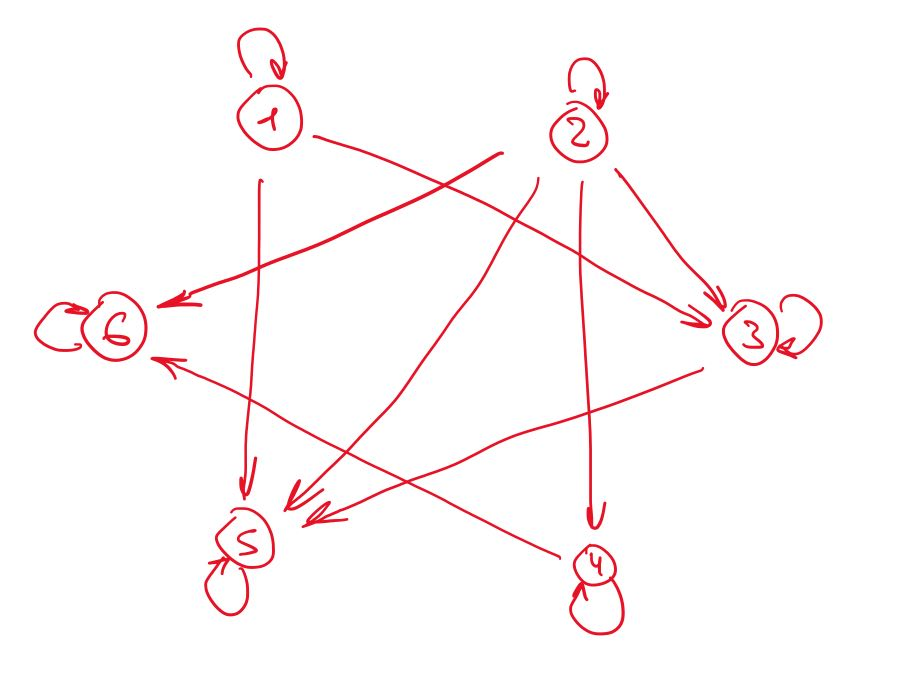
\includegraphics[scale=0.3]{media/graph.jpg}
	 	\caption{Directed graph representing the partial order}
	 	\label{fig:graph}
	 \end{figure}
	 \begin{figure}[h]
	 	\centering
	 	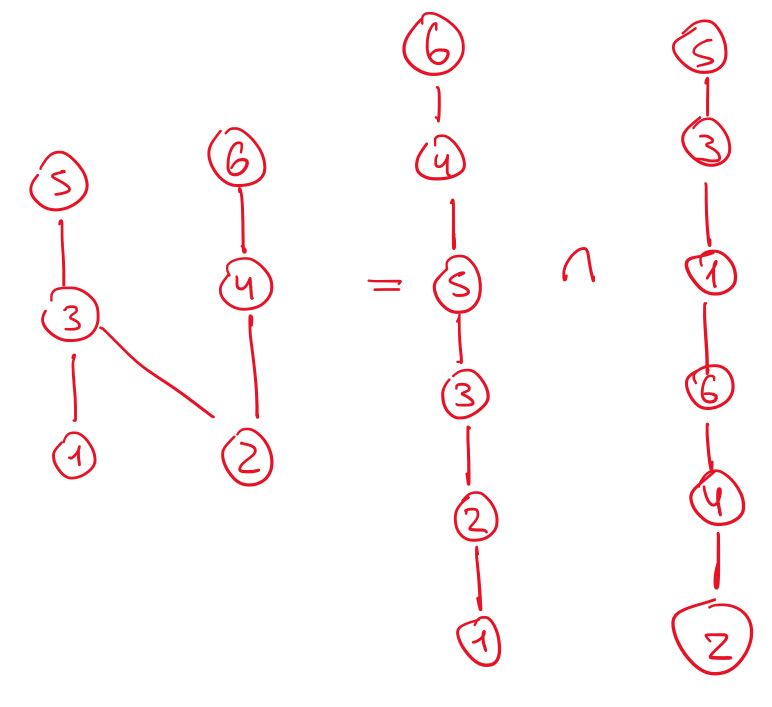
\includegraphics[scale=0.3]{media/hasse.jpg}
	 	\caption{Hasse diagram of the partial order and it's decomposition into an intersection of linear orders}
	 	\label{fig:hasse}
	 \end{figure}
	 \newpage
	 \begin{figure}[h]
	 	\centering
	 	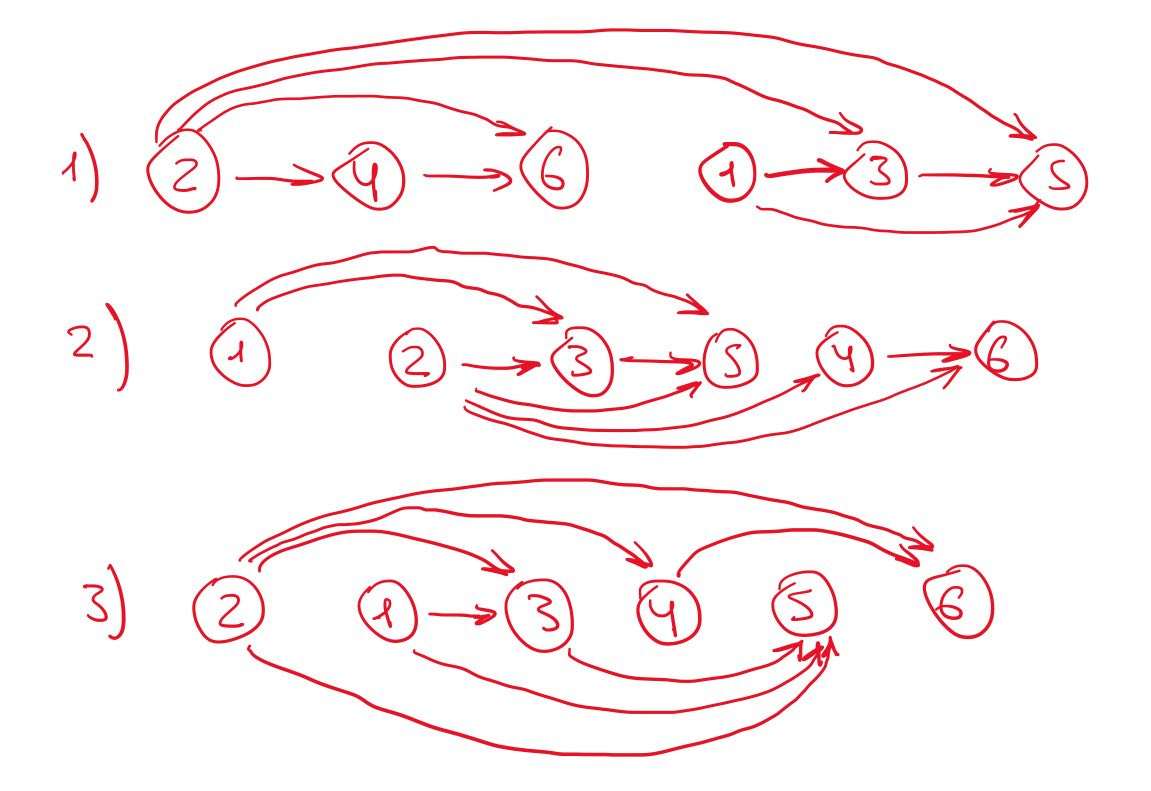
\includegraphics[scale=0.3]{media/toposort.jpg}
	 	\caption{Three different topological sorts for the graph on \figref{fig:graph}}
	 	\label{fig:toposort}
	 \end{figure}
	 
	 \subsection*{Question 3}
	 
	 \noindent\textbf{Task.} Prove that in any arbitrary undirected graph, the number of vertices with odd degree is even.\\
	 
	 \begin{proof} 
	 Let $G=(V,\, E)$ be an undirected graph, where $V$ is the set of its vertexes and $E$ --- the set of its edges. It is a well-known fact that
	 \begin{equation}\label{eq:sum_deg}
		 \sum\limits_{v\in V}\text{deg}(v) = 2|E|,
	 \end{equation}
	 where $\text{deg}(v)$ is degree of a vertex $v\in V$ and $|E|$ is the number of edges in~$G$. Let us suppose that the number of vertices with odd degree is odd. Then $\sum\limits_{v\in V}\text{deg}(v)$ must also be an odd number. This contradicts \ref{eq:sum_deg}, hence the number of vertices with odd degree must be even.\qed
	 \end{proof}
	 \newpage
	 
	 \subsection*{Question 4}
	 
	 \begin{theorem}
	 	Let $(P,\leq_p)$ and $(Q,\leq_q)$ be finite posets with covering relations $\prec_p$ and $\prec_q$, and let $\varphi : P \rightarrow Q$ be a bijection. Then the following two statements are equivalent: 
	 	\begin{enumerate}
	 	\item Bijection $\varphi$ is an order isomorphism, i.e., $x\leq_p y$ iff $\varphi(x) \leq_q \varphi(y)$. 
	 	\item $x \prec_p y$ iff $\varphi(x) \prec_q \varphi(y)$.
	 	\end{enumerate}
	 \end{theorem}
	 
	 \noindent\textbf{Task.} Prove the set of all positive integer divisors of the number 30 with the relation \textit{"to be a divisor"} as an order relation is isomorphic to the set of all subsets $\{x,\, y,\, z\}$ ordered by inclusion.\\
	 
	 \begin{proof}
	 	Let $S = \{x,\, y,\, z\}$ and 
	 	\[\mathbb{P}(S)=\{\{\emptyset\},\,\{x\},\,\{y\},\,\{z\},\,\{x,\, y\},\,\{x,\, z\},\,\{y,\, z\},\,\{x,\, y,\, z\}\}\]
	 	be the powerset(set of all subsets) over it. The set of all positive integer divisors of the number 30 is
	 	\[D_{30}=\{1,\,2,\,3,\,5,\,6,\,10,\,15,\,30\}.\]
	 	Partial order on poset $(D_{30}, |)$ is defined by a following table:
	 	\begin{center}
	 		\begin{tabu}{ |X[c]|X[c]|X[c]|X[c]|X[c]|X[c]|X[c]|X[c]|X[c]|}
	 			\hline
	 			& 1 & 2 & 3 & 5 & 6 & 10 & 15 & 30\\
	 			\hline
	 			1 & 1 & 1 & 1 & 1 & 1 & 1 & 1 & 1\\
	 			\hline
	 			2 &  & 1 &  &  & 1 & 1 &  & 1\\
	 			\hline
	 			3 &  &  & 1 &  & 1 &  & 1 & 1\\
	 			\hline
	 			5 &  &  &  & 1 &  & 1 & 1 & 1\\
	 			\hline
	 			6 &  &  &  &  & 1 &  &  & 1\\
	 			\hline
	 			10 &  &  &  &  &  & 1 &  & 1\\
	 			\hline
	 			15 &  &  &  &  &  &  & 1 & 1\\
	 			\hline
	 			30 &  &  &  &  &  &  &  & 1\\
	 			\hline
	 		\end{tabu}
	 	\end{center}
	 	\pagebreak
	 	Let us consider the table that defines partial order on poset $(\mathbb{P}(S), \subseteq)$ as well:
	 	\begin{center}
	 		\begin{tabu}{ |X[c]|c|c|c|c|X[c]|X[c]|X[c]|X[c]|}
	 			\hline
	 			& $\{\emptyset\}$ & $\{x\}$ & $\{y\}$ & $\{z\}$ & $\{x,\, y\}$ & $\{x,\,z\}$ & $\{y,\, z\}$ & $\{x,\, y,\, z\}$\\
	 			\hline
	 			$\{\emptyset\}$ & 1 & 1 & 1 & 1 & 1 & 1 & 1 & 1\\
	 			\hline
	 			$\{x\}$ &  & 1 &  &  & 1 & 1 &  & 1\\
	 			\hline
	 			$\{y\}$ &  &  & 1 &  & 1 &  & 1 & 1\\
	 			\hline
	 			$\{z\}$ &  &  &  & 1 &  & 1 & 1 & 1\\
	 			\hline
	 			$\{x,\, y\}$ &  &  &  &  & 1 &  &  & 1\\
	 			\hline
	 			$\{x,\,z\}$ &  &  &  &  &  & 1 &  & 1\\
	 			\hline
	 			$\{y,\, z\}$ &  &  &  &  &  &  & 1 & 1\\
	 			\hline
	 			$\{x,\, y,\, z\}$ &  &  &  &  &  &  &  & 1\\
	 			\hline
	 		\end{tabu}
	 	\end{center}
	 	From those tables Hasse diagrams(\figref{fig:hasse_q4}) can be constructed. 
	 	
	 	\begin{figure}[h]
	 		\centering
	 		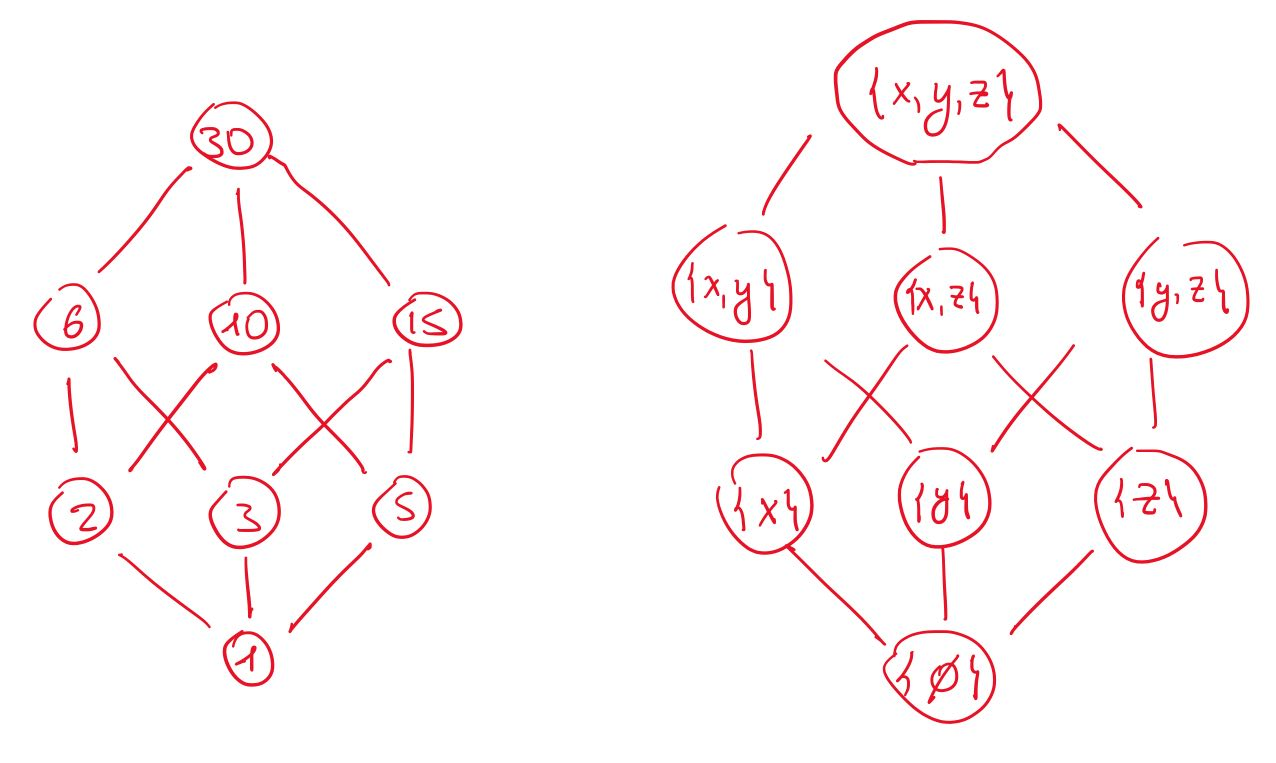
\includegraphics[scale=.27]{media/hasse_q4.jpg}
	 		\caption{Hasse diagrams of $(D_{30},|)$ (left) and $(\mathbb{P}(S), \subseteq)$ (right)}
	 		\label{fig:hasse_q4}
	 	\end{figure}
	 	
	 	If we define a relation $\psi:D_{30}\rightarrow\mathbb{P}(S)$ so that
	 	\begin{multline*}
	 		\psi(1)=\{\emptyset\},\,\psi(2)=\{x\},\,\psi(3)=\{y\},\,\psi(5)=\{z\},\,\psi(6)=\{x,\, y\},\\\psi(10)=\{x,\, z\},\,\psi(15)=\{y,\, z\},\,\psi(30)=\{x,\, y,\, z\},
	 	\end{multline*}
	 	then $(D_{30},|)$ and $(\mathbb{P}(S), \subseteq)$ along with $\psi$ satisfy the conditions for theorem 1, thus they are isomorphic.\qed
	\end{proof}
	\newpage
	
	\subsection*{Question 5}
	
	\noindent\textbf{Task.} For the binary relation $(\{1, 2, 3, 4, 6, 24, 36, 72\},|)$:
	\begin{enumerate}
		\item Prove that it is a partial order. 
		\item Draw its diagram. 
		\item Using the diagram, find the following:
		\begin{enumerate}
			\item Maximal elements. 
			\item Largest element (Maximum). 
			\item Minimal elements. 
			\item Least element (Minimum). 
			\item $\downarrow\{4,\, 6\}$
			\item $\uparrow\{4,\, 6\}$ 
			\item $\downarrow\{3,\, 4\}$ 
			\item $\uparrow\{3,\, 4\}$ 
			\item $\downarrow\{36,\, 24\}$
			\item $\uparrow\{36,\, 24\}$
		\end{enumerate}
	\end{enumerate}
	
	\noindent\textbf{Solution.} Let us denote $\{1,\, 2,\, 3,\, 4,\, 6,\, 24,\, 36,\, 72\}$ as $A$. Consider the relation table for $(A,\,|)$.
	
	\begin{center}
		\begin{tabu}{ |X[c]|X[c]|X[c]|X[c]|X[c]|X[c]|X[c]|X[c]|X[c]|}
			\hline
			& 1 & 2 & 3 & 4 & 6 & 24 & 36 & 72\\
			\hline
			1 & 1 & 1 & 1 & 1 & 1 & 1 & 1 & 1\\
			\hline
			2 &  & 1 &  & 1 & 1 & 1 & 1 & 1\\
			\hline
			3 &  &  & 1 &  & 1 & 1 & 1 & 1\\
			\hline
			4 &  &  &  & 1 &  & 1 & 1 & 1\\
			\hline
			6 &  &  &  &  & 1 & 1 & 1 & 1\\
			\hline
			24 &  &  &  &  &  & 1 &  & 1\\
			\hline
			36 &  &  &  &  &  &  & 1 & 1\\
			\hline
			72 &  &  &  &  &  &  &  & 1\\
			\hline
		\end{tabu}
	\end{center}
	
	For a binary relation to be a partial order, it must be reflexive, antisymmetric and transitive. Since the table consists of upper triangular matrix, $\forall x\in A \,\,\, x|x$ and $\forall x,\, y \in A \,\,\, x|y \implies \lnot y|x$, therefore the relation is reflexive and antisymmetric. Let us consider matrix
	\[M=\left(m_{ij}\right)=\begin{pmatrix}
		1 & 1 & 1 & 1 & 1 & 1 & 1 & 1\\
		0 & 1 & 0 & 1 & 1 & 1 & 1 & 1\\
		0 & 0 & 1 & 0 & 1 & 1 & 1 & 1\\
		0 & 0 & 0 & 1 & 0 & 1 & 1 & 1\\
		0 & 0 & 0 & 0 & 1 & 1 & 1 & 1\\
		0 & 0 & 0 & 0 & 0 & 1 & 0 & 1\\
		0 & 0 & 0 & 0 & 0 & 0 & 1 & 1\\
		0 & 0 & 0 & 0 & 0 & 0 & 0 & 1\\
	\end{pmatrix},\]
	where zeros correspond to empty cells in the relation table. Its matrix product with itself is
	\[V = \left(v_{ij}\right) = M^2 =\begin{pmatrix}
		1 & 2 & 2 & 3 & 4 & 6 & 6 & 8\\
		0 & 1 & 0 & 2 & 2 & 4 & 4 & 6\\
		0 & 0 & 1 & 0 & 2 & 3 & 3 & 5\\
		0 & 0 & 0 & 1 & 0 & 2 & 2 & 4\\
		0 & 0 & 0 & 0 & 1 & 2 & 2 & 4\\
		0 & 0 & 0 & 0 & 0 & 1 & 0 & 2\\
		0 & 0 & 0 & 0 & 0 & 0 & 1 & 2\\
		0 & 0 & 0 & 0 & 0 & 0 & 0 & 1\\
	\end{pmatrix}.\]
	Here, according to the definition of matrix product, $v_{ij} = \sum\limits_{k=1}^{n}m_{ik}m_{kj}$, where $n$ is size of the matrix $M$. Therefore, $v_{ij}>0$ iff there is a two-step path between $i$ and $j$ and the value of $v_{ij}$ is the number of two-step paths between $i$ and $j$. 
	
	The relation is transitive, if there no pair of incomparable elements with a two-way path between them:
	\[\nexists i,\, j: \,\,\, m_{ij} = 0\land\, v_{ij} > 0.\]
	Since there are no elements that do not satisfy this condition, the relation $(A,\,|)$ is also transitive, therefore it is a partial order.
	
	\newpage
	Let us consider its Hasse diagram:
	
	\begin{figure}[h]
		\centering
		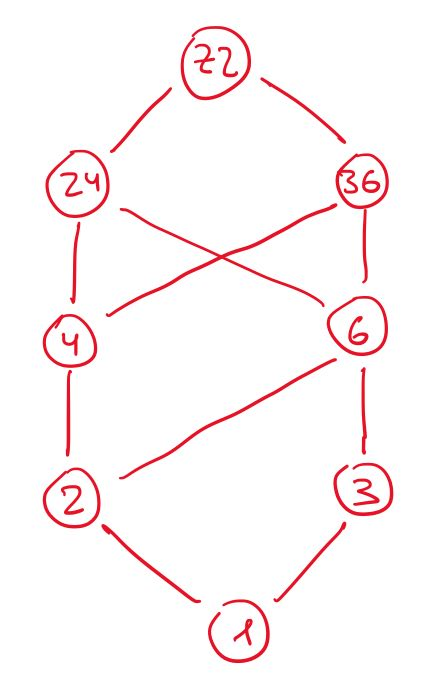
\includegraphics[scale=0.3]{media/hasse_q5.jpg}
		\caption{Hasse diagram of the partial order $(A,\,|)$}
		\label{fig:hasse_q5}
	\end{figure}
	
	
	\noindent using it, we can determine that:
	\begin{enumerate}
		\item The set of maximal elements consists only of 72. 
		\item The maximum is 72. 
		\item The set of minimal elements consists only of 1.  
		\item The minimum is 1. 
		\item $\downarrow\{4,\, 6\} = \{4,\, 6,\, 2,\, 3,\, 1\}$
		\item $\uparrow\{4,\, 6\} = \{4,\, 6,\, 24,\, 36,\, 72\}$ 
		\item $\downarrow\{3,\, 4\} = \{3,\, 4,\, 2,\, 1\}$ 
		\item $\uparrow\{3,\, 4\} = \{3,\, 4,\, 6,\, 24,\, 36,\, 72\}$ 
		\item $\downarrow\{36,\, 24\} = \{36,\, 24,\, 4,\, 6,\, 2,\, 3,\, 1\}$
		\item $\uparrow\{36,\, 24\} = \{36,\, 24,\, 72\}$
	\end{enumerate}
	\newpage
	
	\subsection*{Question 6}
	
	\noindent\textbf{Task.} Prove that the incomparability relation for a strict order is a tolerance relation.
	
	\begin{proof}
		 Let incomparability relation be denoted as $\nprec$ and the strict order to be defined on some set $S$. A strict order is a antireflexive relation, thus 
		 \[\forall x\in S \,\,\, \lnot x<x \implies x\nprec x.\]
		 so incomparability relation is reflexive. Suppose that incomparability relation is not symmetrical. Then there would be such pair $x,\, y\in S,\, x\neq y$\footnote{We are not considering the case when $x$ and $y$ are the same element, since it was already shown that incomparability relation is reflexive.} that $x\nprec y$ and $\lnot y\nprec x$. Since elements $x$ and $y$ are called incomparable if 
		 \[x\neq y \implies \lnot (x<y\lor y>x),\]
		 this would imply that both $\lnot (x<y\lor y>x)$ and $y<x\lor x>y$, which a contradictory statement. Therefore, incomparability relation is symmetrical, hence it is a tolerance relation.\qed 
	\end{proof}
	
	\subsection*{Question 7}
	
	\noindent\textbf{Q.} Which of the three options have you picked for the big project?\\
	\noindent\textbf{A.} Neural FCA.
\end{document}